\documentclass[10pt,twocolumn,letterpaper]{article}

\usepackage{statcourse}
\usepackage{times}
\usepackage{epsfig}
\usepackage{graphicx}
\usepackage{amsmath}
\usepackage{amssymb}


% Include other packages here, before hyperref.

% If you comment hyperref and then uncomment it, you should delete
% egpaper.aux before re-running latex.  (Or just hit 'q' on the first latex
% run, let it finish, and you should be clear).
\usepackage[breaklinks=true,bookmarks=false]{hyperref}

\statcoursefinalcopy


\setcounter{page}{1}
\begin{document}


%%%%%%%%%%%%%%%%%%%%%%%%%%%%%%%%%%%%%%%%%%%%%%%%%%%%%%%%%%%%%%%
% DO NOT EDIT ANYTHING ABOVE THIS LINE
% EXCEPT IF YOU LIKE TO USE ADDITIONAL PACKAGES
%%%%%%%%%%%%%%%%%%%%%%%%%%%%%%%%%%%%%%%%%%%%%%%%%%%%%%%%%%%%%%%



%%%%%%%%% TITLE
\title{ SBE304 Project Proposal}

\author{First Author\\
{\tt\small mr.adel98@hotmail.com}
\and
Second Author\\
{\tt\small engmohamedyasser8@gmail.com}
\and
Third Author\\
{\tt\small iomar9606@gmail.com}
\and
Fourth Author\\
{\tt\small MuhammedMohsen1111@gmail.com}
}

\maketitle
%\thispagestyle{empty}



% MAIN ARTICLE GOES BELOW
%%%%%%%%%%%%%%%%%%%%%%%%%%%%%%%%%%%%%%%%%%%%%%%%%%%%%%%%%%%%%%%



%%%%%%%%% BODY TEXT



%\begin{itemize}

%	\item This template is based on the CVPR conference template\footnote{\url{http://statcourse2018.thecvf.com/submission/main_conference/author_guidelines}}.
	
%	\item The information in this template is very minimal, and this file should serve you as a framework for writing your proposal. You may prefer to use a more collaboration-friendly tool while drafting the report with your class mates before you prepare the final report for submission. Remember that you should \textbf{submit both the report and code} you used for this project via Canvas. Also, \textbf{only one member per team} needs to submit the project material.
	
%	\item The project proposal is a 2-4 page document excluding references\footnote{This means, references should of course be included but do not count towards the page limit}.
	
%	\item You are encouraged (not required) to use 1-2 figures to illustrate technical concepts.
	
	%\item The proposal must be formatted and submitted as a PDF document on Canvas (the submission deadline will be later announced via the schedule \& email).
	
	%\item Please
	%check out the text in these sections for further information.
	
%\end{itemize}




\section{Introduction}


%In this section, describe what you are planning to do. Also, briefly describe related work.


%When discussing related work, do not forget to include appropriate references.  This is an example of a citation \cite{mirjalili2018gender}. To format the citations properly, put the
%corresponding references into the bibliography.bib file. You can obtain
%BibTeX-formatted references for the "bib" file from Google Scholar 
%(\url{https://scholar.google.com}), for example, by clicking on the 
%double-quote character under a citation and then selecting \mbox{"BibTeX"} as
%shown in Figure \ref{fig:google-scholar-1col} and 
%Figure \ref{fig:google-scholar-2col}.


%\begin{figure}[t]
%\begin{center}
 %  
\includegraphics[width=0.8\linewidth]{figures/google-scholar.pdf}
%\end{center}
  % \caption{Example illustrating how to get BibTeX references from
 % Google Scholar as a 1-column figure.}
%\label{fig:google-scholar-1col}
%\end{figure}


%\begin{figure*}
%\begin{center}
 %  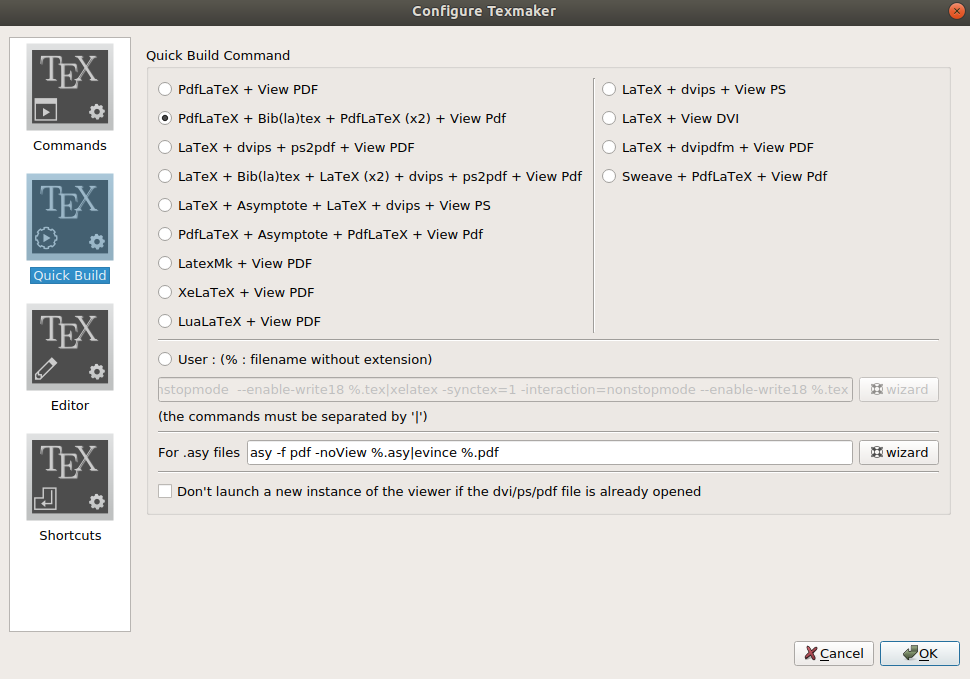
\includegraphics[width=0.8\linewidth]{figures/config-texmaker.png}
%\end{center}
 %  \caption{Compiling this document using \emph{TexMaker}.}
%\label{fig:google-scholar-2col}
%\end{figure*}
\textbf{\textit{Project objective:}} the aim of this project is to estimate the survival rate characteristics of 165 hepatocellular carcinoma (HCC) patients and identify useful prognostic factors to help in the clinical management of patients with (HCC). this project is important because according to "Hebei Medical University in China" the median survival time is 1, 2, 3, and 5 year survival rates equal to 49.3\%, 35.3\%, 26.6\%, and 19.5\% respectively. The results showed that the Barcelona clinic liver cancer (BCLC) stage and Tumor size were independent prognostic factors to HCC patients. The survival rate of HCC patients has increased in the recent years, at the same time the overall survival rate and the prognosis were poor\cite{wang2019clinical}. \\  
\textbf{\textit{Our work:}} we will do prepossessing on the data-set   using:(feature selection, feature normalization, and data imputation) for 165 patient with HCC before starting, so our result will be accurate, and get a good overall view about the survival rate of HCC patients, we have selected three appropriate methods for our project:(KNN model, NB classifier, and Logistic regression) and we will compare the result to get the most accurate method.

\section{Motivation}

with more than 600000 deaths a year,HCC is one of the most common cancers in the world.\\ in Egypt it represents  the second most common cancer in men and the 6th most common cancers in women \cite{omar2013risk}.\\
Geographical distribution of HCC varies throughout the world with an incidence rate ranging from 2.1 in Central America to 35.5 in Eastern Asia.\\
The burden of HCC has been increasing in Egypt with a doubling in the incidence rate in the past 10 years,mostly due to high prevalence of viral hepatitis and its complications,
Also There is a geographic correlation between the incidence of HCC and the prevalence of chronic hepatitis B and C, suggesting that these two viral infections are the most important risk factors of HCC worldwide.\\
And as we know Egypt is the $1^{st}$ country in the world regarding HCV prevalence , so we want to take a closer look at HCC and the factors that affect it, to provide a useful information that helps the doctors for better understanding of the HCC and what affect it's survival rate,and also we hope this information help the government to put a well thought out plan for raise awareness about HCC.; and there lies our motivation.\\
  
 


\section{Evaluation}

%What would the successful outcome of your project look like? In other words, under which circumstances would you consider your project to be “successful?”

%How do you measure success, specific to this project, from a technical standpoint?
in our point of view a successful outcome of this project is to be able to predict whether the patient dies or not,i.e to be able to interpret the data to useful information after applying the chosen methods to it.   
\section{Resources}

What resources are you going to use (datasets, computer hardware, computational tools, etc.)?

\section{Preprocessing}
\begin{itemize}
	\item Feature selection:\\
	we will remove any redundant feature (if there is any ) by calculating the correlation matrix and removing feature with correlation -ideally- of 0.75 or higher.\\this will be done using Caret R package.\\
	\item Feature normalization:\\
	we will rescale the features so they will have a distribution with $\sigma=1$ and $\mu=0$\\this is a general requirement for many machine learning algorithms .\\this will be done using Z-Score Standardization technique using the built-in function in R (scale()).\\
	
	\item Data imputation:\\
	we will use PMM  imputation,to over come the problem of the missing values in our data.\\
\end{itemize}

\section{EDA}
\begin{itemize}
	
	\item The Heat Map procedure shows the distribution of a quantitative variable over all combinations of 2 categorical factors. If one of the 2 factors represents time, then the evolution of the variable can be easily viewed using the map. A gradient color scale is used to represent values of the quantitative variable and there is an example for it.
\begin{figure}[h]
\centering
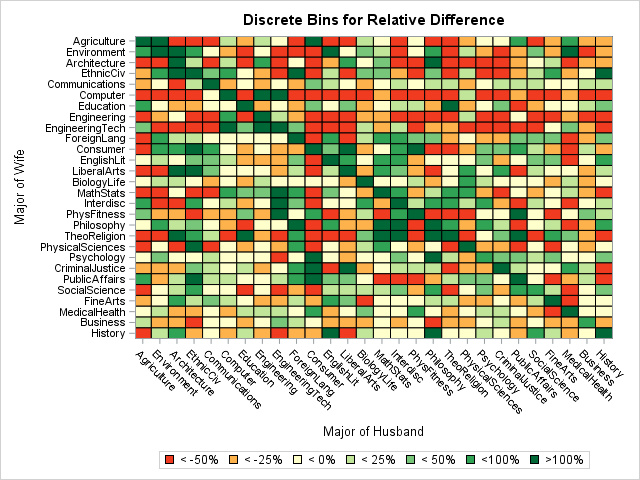
\includegraphics[width=0.35\textwidth]{a2}
\caption{Heat Map}
\label{Figure1:a2}
\end{figure}
	\item The Violin Plot Statlet displays data for a single quantitative sample using a combination of a box-and-whisker plot and a nonparametric density estimator. It is very useful for visualizing the shape of the probability density function for the population from which the data came. A separate procedure is available for creating violin plots for multiple samples and there is an example for it.
\begin{figure}[h]
\centering
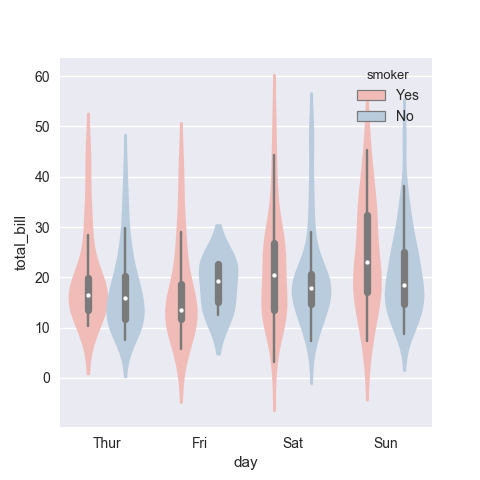
\includegraphics[width=0.35\textwidth]{a3}
\caption{Violin Plot}
\label{Figure2:a3}
\end{figure}

\end{itemize}


\section{Contributions $\&$ Timetable }

table of tasks to be done and its date.\\ 
\begin{table}[h]
	\centering
	\begin{tabular}{|c|c|}
	\hline
	TASK & Date\\
	\hline
	Apply pre-processing and EDA to the data  & 31\textbackslash 10 to 2 \textbackslash 11 \\
	\hline
	Learn and apply NB classifier to the data & 3\textbackslash 11 to 6\textbackslash 11  \\
	\hline
	Learn and apply KNN model to the data & 7\textbackslash 11 to 10\textbackslash 11\\
	\hline
	Learn and apply logistic regression to the data& 11\textbackslash 11 to 14\textbackslash 11\\
	\hline
	revision and editing & 22\textbackslash 11 \\
	\hline
	submitting the prototype & 25\textbackslash 11\\
	\hline
	\end{tabular}
\end{table}
%You are expected to share the workload evenly, and every group member is expected to participate in both the experiments and writing. (As a group, you only need to submit one proposal and one report, though. So you need to work together and coordinate your efforts.)
%Clearly indicate what computational and writing task each member of your group will be participating in.



\section{Chosen methods}
\begin{itemize}
	\item NB classifier.\\
	\item KNN model.\\
	\item Logistic regression.\\
\end{itemize}

\section{Websites}
\begin{itemize}
	\item \href{https://adelmoustafa098.github.io/indigo/}{Adel Moustafa}\\
	\item \href{https://oimas.github.io}{Omar Ibrahim} \\
	\item \href{https://engmohamedyasser8.wixsite.com/mohamedyasser?fbclid=IwAR13NXjthxdr0YZe5gdpg0rbowpzE36lq2x7HdTIMUuPkDaKITjwjJiWi1E}{Mohammed Yasser} \\
	\item \href{https://muhammedmohsn.github.io/MuhammedMohsn.git.io-/}{Muhammed Mohsen} \\
\end{itemize}

	

{\small

\bibliographystyle{IEEEtran}
\bibliography{bibliography.bib}
\begin{itemize}

	\item Gastroenterology $\&$ Hepatology-HCC Burden in Egypt.\\
\end{itemize}

}

\end{document}
